
\chapter{Onderzoek: Methode en tooling voor SOUP-analyses binnen Eaglescience}\label{ch:onderzoek-tool-methode}
In het vorige hoofdstuk is duidelijk geworden dat er veel externe bibliotheken worden gebruikt om applicaties te ontwikkelen. Veel bedrijven kunnen niet meer zonder en Eaglescience is hier geen uitzondering op. Het gebruik van externe bibliotheken heeft te veel voordelen op het gebied van besparing(tijd en geld), flexibiliteit, standaardisering om te proberen om deze voordelen te benutten middels intern ontwikkelde projecten. Het gebruik van externe bibliotheken is echter niet zonder gevaren en zonder dat er maatregelen worden genomen kunnen er kwetsbaarheden worden gebruikt om informatie of functionaliteit binnen een applicatie te misbruiken door kwaadwillenden. Er bestaan bronnen zoals de NVD van het NIST waarin deze kwetsbaarheden worden opgeslagen. Het is echter ondoenlijk om deze database met de hand te doorzoeken. Zeker op het moment dat de applicaties dusdanig veel bibliotheken gebruiken dat het volume te groot wordt. Volgens de aanwijzingen vermelding in de OWASP-top10 dienen alle dependencies en de geneste dependencies gecontrolleert te worden.

Dit onderzoek gaat over het zoeken van tooling en methoden om deze analyse automatisch en periodiek te kunnen doen om zo inzichtelijk te maken of er kwetsbaarheden in de uitgerolde applicatie zitten. Met het gebruiken van deze methode hoeft alleen de applicatie nog maar met de hand up-to-date te worden gehouden. Dit laatste is door de complexiteit bewust uit de opdracht gehouden. De onderzoeksvraag is dan ook: "Welke SCA tooling is compabitble met de omgeving van Eaglescience en welke methode kan worden toegepast om deze tooling te gebuiken voor het automatisch analyseren van externe dependencies?". De hoofdvraag werpt de volgende deelvragen op die ieders hieronder worden beantwoord in een eigen paragraaf waarna een in de conclussie de methode wordt aangeboden.
\begin{itemize}
    \item Welke Werkwijze en Dev-stack gebruikt Eaglescience voor het ontwikkelen van software?
    \item Hoe wordt er op dit moment software uitgerold binnen Eaglescience?
    \item Wat zijn de selectiecriteria voor tools die gebruikt kunnen worden?
    \item Welke tools zijn er beschikbaar?
    \item Hoe zijn deze tools te intgreren in de huidige buildstraat van Eaglescience?
    \item Welke methode kan worden gebruikt om middels de gevonden tools informatie over kwetsbaarheden binnen externe bibliotheken te vinden?
\end{itemize}

\section{Werkwijze en Dev-stack binnen Eaglescience}\label{sec:werkwijze-en-dev-stack-binnen-eaglescience}
Voordat er kan worden onderzocht welke tools en methode er geschikt zijn om een analyse te doen op projecten die Eaglescience in haar beheer heeft dient er gekeken te worden naar de manier waarop zij werkt en met welke middelen projecten worden ontwikkeld. Deze kennis is nodig om de een scope aan te brengen in de zoektoch naar tooling.

\subsection{Werkwijze}\label{subsec:ESwerkwijze}
Binnen Eaglescience wordt er geprobeerd om "full Scrum" te werken. Dit wil zeggen dat voor ieder project een team van maximaal 9 full-stack developers wordt aangewezen. De sprints duren ongeveer 2 á 3 weken afhankelijk van wensen van de klant en beschikbaarheid van ontwikkelaars. Iedere sprint begint met een refinement waarbij de taken die op de backlog staan worden bekeken en ingeschat door het team. Tijdens de sprint vindt de ontwikkeling middels taken plaats die vervolgens worden gereviewd door een ander teamlid. Aan het einde van de sprint vind er een retrospective plaats en eventueel een demo om de voortgang te demonstreren aan de klant, dit is ook het moment dat het team ziet hoe de applicatie in het algemeen werkt. Dit is ook het moment voor de projectmanager en product owner om de taken die op de back-log staan opnieuw te prioriseren waarbij in de refinement van de volgende sprint de taken mee worden genomen.

\subsection{Dev-stack}\label{subsec:ESdev-stack}
EagleScience maakt volledige full stack oplossingen. Er wordt dus zowel front-end, backend, en database oplossingen ontwikkelt binnen projecten. Om deze reden wordt er binnen EagleScience gebruik gemaakt van verchillende ontwikkeltalen en tooling om projecten te voltooien. Hieronder staan de belangrijkste vermeld. Deze lijst is bij lange na niet volledig.

\subsubsection{OntwikkelTalen en frameworks}\label{subsec:ontwikkeltalen-en-frameworks}
Zoals eerder beschreven ontwikkelend EagleScience software full-stack. Er wordt dus gebruik gemaak van zowel talen voor de frontend en backend. Databases worden niet meegenomen in de lijst omdat deze als complete componenten worden gezien en de analyse op SOUP in deze ook niet veel zin heeft.
\begin{itemize}
    \item \textbf{Backend} De voornamelijkst taal voor het ontwikkelen van de backend binnen EagleScience is Scala. De keuze voor deze taal is de mogelijkheid om functioneel te kunnen programmeren in de Java Virtual Machine(JVM). Dat laatste zorgt ervoor dat bibliotheken die geschreven zijn in talen die ook ondersteunt worden door de JVM gebruikt kunnen worden door Scala. Daarbij heeft Scala de mogelijkheid om naadloos mee te groeien met een project. Vandaar de naam Scala wat een samenraapsel is van Scalable Language. De ondersteuning voor functioneel programeren geeft het voordeel dat de geschreven code makkelijker te testen is wat toe te dragen is aan het gebruik van pure functies. Pure functies hebben de eigenschap deterministisch te zijn wat wil zeggen dat iedere keer als een bepaalde input in een functie komt er altijd dezelfde output verwacht kan worden, zonder dat er side-effects plaatsvinden die de staat van een applicatie onbedoelt kunnen veranderen, wat de betrouwbaarheid ten goede komt. Deze eigenschap maakt het mogelijk om applicaties sneller en makkelijker te testen. Binnen EagleScience worden er in bijna alle projecten een aantal frameworks/bibliotheken gebruikt die het ontwikkelen van microservice web applicaties in Scala makkelijker maakt:
    \begin{itemize}
        \item \textbf{PlayFramework 2.xx} Een web framework voor de ontwikkeling van webapplicaties in Scala we gebruikten het vooral als router voor de verschillende microservices die er achterliggen.
        \item \textbf{ArchES} is een intern ontwikkeld framework wat de opbouw en de communicatie tussen microservices in scala verbeterd.ArchES is geinspireerd op Apache KAFKA en werkt middels hetzelfde pub -> sub principe.
    \end{itemize}
\end{itemize}
Binnen Scala kan er gebruik gemaakt worden van enkele buildtools zoals Maven, Gradle en Scala Build Tool (SBT). Binnen EagleScience wordt SBT gebruikt. Dit omdat het de defacto tool is voor Scala.
[NOTE: dependency declaraties toe voegen?]

\subsubsection{Frontend}
Voor de frontend wordt veelvuldig gebruik gemaakt van TypeScript, een extensie op Javascript. Het meeste gebruikte frameworks is Angular welke gebruikt wordt om de diverse portalen en Unser-interfaces te ontwikkelen. NativeScript wordt gebruikt in combinatie met Angular om voor Mobile apps te kunnen ontwikkelen. TypeScript maakt het mogelijk om in javascript getypeert te programeren wat kan garanderen dat tijdens bugs en andere fouten tijdens het ontwikkelen opgemerkt kan worden zodat deze niet pas tijdens run-time aan het ligt komen. De reden voor het gebruik van Nativescript is dat het de mogelijkheid geeft om Angular te gebruiken voor de ontwikkeling van zowel android als IOS apps.  Beide ontwikkelframeworks draaien in JavaScript en om die reden is Node.js gebruikt als ontwikkelomgeving. En gezien javascript niet gecombileerd en dus niet gebuild wordt is er alleen een voorziening voor dependency management in de form van Yarn en Node Package Manager(NPM). Binnen EagleScience wordt NPM
gebruikt voor het beheer van dependencies in een project.


\subsubsection{Tooling}\label{subsec:tooling}
Naast ontwikkeltalen gebruikt EagleScience een aantal tools om dagelijkse werkzaamheden te stroomlijnen en software uit te rollen voor de klant. De tools zijn ieder op zijn beurt verantwoordelijk voor een specifieke taak en alle projecten dienen gebruik te maken van deze tools waar gepast. Hoe de tools samenwerken en uitgerold zijn is te zien in figuur~\ref{fig:es-tooling}

\begin{itemize}
    \item \textbf{Jira} Binnen EagleScience wordt Jira gebruikt om taken binnen projecten te beheren. Hier worden taken aan projecten toegevoegd welke vervolgens in een spring wordt opgenomen. Deze sprints worden ook beheert middels Jira
    \item \textbf{Confluence}
    Confluence wordt gebruikt voor het documenteren van de verschillende projecten waar EagleScience aan werkt. Confluence en Jira zijn beiden van Atlassian wat ervoor zorgt dat deze met elkaar kunnen communiceren wat op zijn beurt de documentatie verbeterd. Op dit moment lijkt het erop dat Confluence een end of life heeft on 2023 en dat voor dit systeem een vervanging moet worden gevonden.
    \item \textbf{GitLab}
    Gitlab wordt binnen EagleScience gebruikt als Version control systeem. Er is voor gekozen om deze on premise te gebruiken op een server in eigen beheer op locatie. Gitlab biedt naast version control ook andere tooling aan die het mogelijk maken om vanuit gitlab te builden en/of uit te rollen echter wordt dit binnen EagleScience gedaan middels een andere tool genaamd Jenkins.
    \item \textbf{Jenkins}
    Jenkins is een open-source automation server wat door Eaglescience gebruikt wordt om projecten te builden, testen, en deployen. Jenkins is gebouwd op een Java omgeving en is daarom uitermate geschikt om met gradle, Maven en SBT projecten om te gaan. Daarnaast kan het middels diverse Shellscripts (Bash, SH, PowerShell) aanverwante taken uitvoeren. Als laatst kan het middels plugins ook uitrollen op cloud omgevingen. Om deze redenenen heeft EagleScience gekozen om Jenkins te gebruiken. In een sectie hieronder wordt uitvoerig uitgewijd over hoe Jenkins binnen EagleScience een project build, test en uitrold.
    \item \textbf{Portal} Een medewerkers portal welke op het moment van schrijven aan ontwikkeld wordt om tools en gegevens aan te bieden die niet project specifiek zijn. Op dit moment wordt er een LDAP password reset tool en verlof inzage en aanvraag aangebonden. Er wordt naast de module voor SOUP analyses ook een modele ontwikkeld welke het mogelijk maakt om uren te registreren. Deze ontwikkelingen zijn een antwoord op de wens om systemen samen te voegen om zo een overzichtelijker geheel aan te bieden voor werknemers.

    \begin{figure}
        \centering
        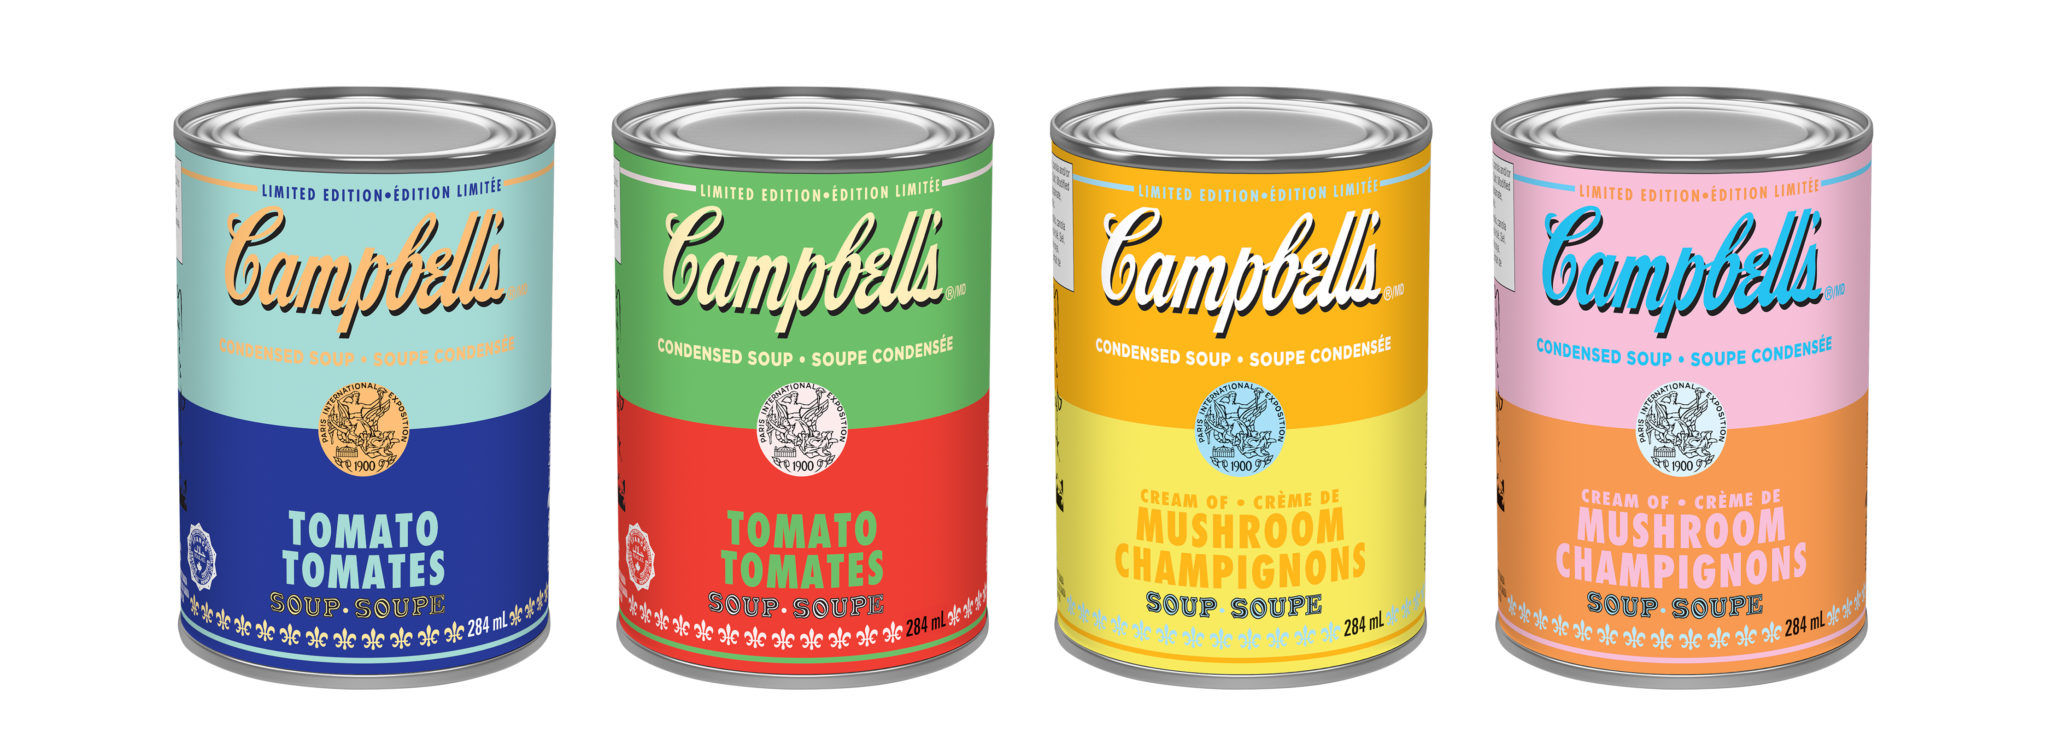
\includegraphics[width=10cm]{gfx/soupcans}
        \caption{Deze nog maken}
        \label{fig:es-tooling}
    \end{figure}

\end{itemize}
%TODO: Nalopen
\section{Hoe wordt op dit moment software gedeployed?}\label{sec:hoe-wordt-op-dit-moment-software-gedeployed?}
Zoals hierboven berschreven wordt Jenkins gebruikt om software te deployen naar zowel de productie omgevingen alsook de verschillende development en acceptatie omgevingen.
Een deploy wordt gedaan op het moment dat er source code naar gitlab gepushed wordt.
Doormiddel van Tokens in de Commit message kan gestuurd worden waar de build(als deze slaagt) gedeployed wordt bijv: {-all + portal} build en deployed alleen de portal. [ci-skip] zorgt ervoor dat er alleen een push wordt gedaan en geen build wordt gestart.
De configuratie die Jenkins gebruikt wordt beschreven in een aantal Jenkins files die meegenomen worden de repo. Middels parameters meegegeven in de commit kan er worden beslist of er een build moet plaatsvinden en zo ja waar en welke delen van de applicatie. Op deze manier is er een flexibiliteit voor de ontwikkelaar.
[NOTE Illustratie maken.....]
Naast de deploy geeft Jenkins nog een aantal andere waardevolle Artifacts als test/lint rapportages.
Een build en deploy gaat volgens de onderstaande afbeelding:

\begin{figure}[H]
    \myfloatalign
    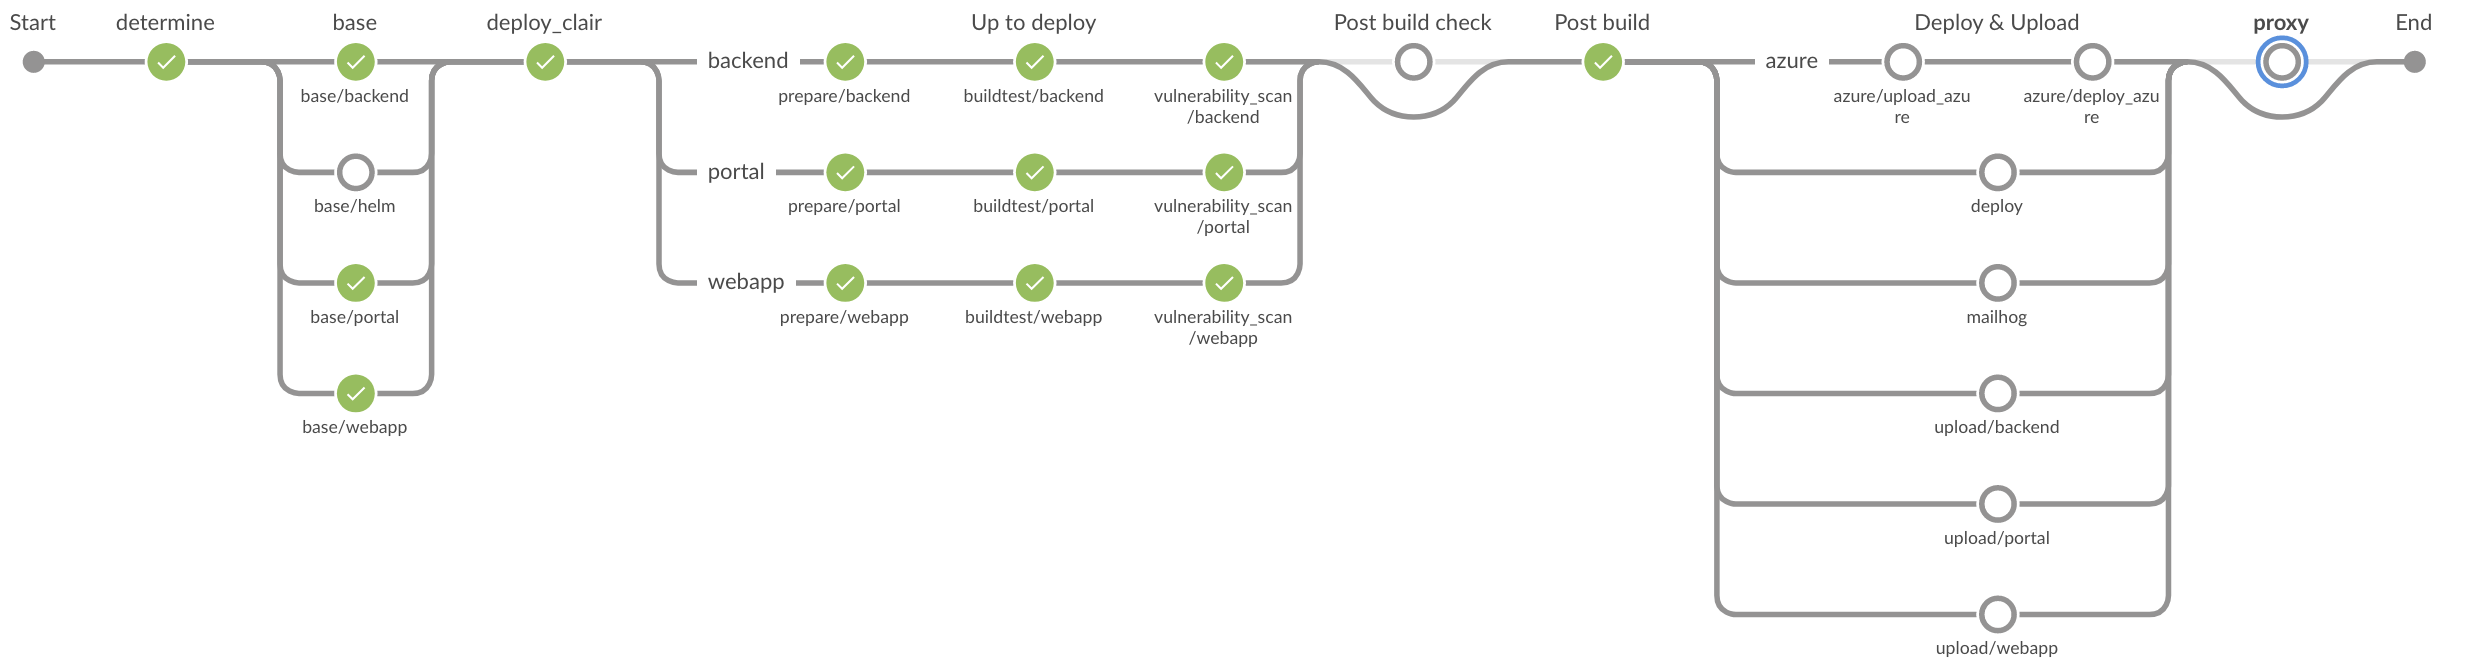
\includegraphics[width=15cm]{gfx/Screenshot 2021-08-18 Jenkins PipeLine}
    \caption{Jenkins(Blue Ocean) pipeline}
    \label{fig:JenkinsPipeLine}
\end{figure}
Een Jenkins pipeline werkt in een aantal stappen dat in een .jenkinsFile wordt beschreven.
Deze jenkinsFile wordt in de determine stap ingelezen en de benodigde stappen op een rij gezet.
De stappen die worden uitgevoerd zijn:
\begin{itemize}
    \item \textbf{determine} Nu wordt bekeken welke stappen er nodig zijn om een succesvolle build en of deploy te kunnen doen./ Aan de hand van een JenkinsFile en tokens in een Commit message wordt hier bekeken welke stappen er moeten worden uitgevoerd om tot een goed einde te komen.
    \item \textbf{base} In de base stap worden alle Containers voorbereid die nodig zijn om de applicatie te draaien.\ Images worden opgehaald en gedeployed De base stap is een parallel lopende stap waarin in dit geval backend, portal en de app worden voorbereid.
    \item \textbf{deploy clair} de clair scanner zoekt op kwetsbaarheden binnen containers die zojuist zijn aangemaakt.\ Dit is een extra veiligheid die ervoor zorgt dat de images en container veilig zijn er alleen nog door bibliotheken die gebruikt worden voor ontwikkeling kwetsbaarheden kunnen worden toegevoegd
    \item \textbf{Up to deploy}
    in dit geval wordt er voor de backend, portal, en app een parallel process gestart waarin alle drie substappen doorlopen:
    \begin{itemize}
        \item \textbf{prepare} Docker containers worden ingesteld, en klaar gezet voor het ontvangen van de services.
        \item \textbf{builtest} De services worden gebuild en gestest in deze stap.\ Eaglescience heeft een aantal tresholds opgesteld waaraan tests moeten voldoen om deze te analyseren worden de test resultaten vanuit de docker containers gekopieerd naar de Jenkins Store waar Jenkins de waarden kan analyseren als alle tests binnen de resultaten vallen wordt de volgende stap uitgevoerd.
        \item \textbf{vulnerability scan} Clair scanner scant nu de containers nogmaals maar nu op de gebruikte software.\ Als clair iets vind dat eaglescience als verdacht acht dan wordt de build gestaakt.
    \end{itemize}
    \item \textbf{PostBuild(check)}
    Alle bevindingen worden hier gecheckt mocht er iets mis zijn wordt er wederom afgebroken en is de build gefaald en kan er dus niet een deploy plaatsvinden.
    \item \textbf{Deploy \& Upload}
    in dit geval wordt de deploy niet uitgevoerd.\ Deze stap zorgt ervoor dat de gebouwde containers worden overgedragen naar Azure.\ Iedere container heeft wederom zijn eigen stappen.
    \item \textbf{End}
    Einde van de PipeLine Jenkins geeft de workers die het project heeft gebruikt weer vrij.
\end{itemize}

\section{Passende SCA tooling en Methode om SOUP-analyses binnen Eaglescience uit te voeren}\label{sec:sca-tooling}
In de opdracht (zie hoofstuk~\ref{ch:opdracht}) staat vermeld dat de te ontwikkelen module eenvoudig gebruikt dient te worden binnen de bestaande CI/CD Pipeline en dat de resultaten zichtbaar moeten zijn in de huidige portal. [NOTE: MEER REDENENEN?] Om deze redenen moet er dus een tool gevonden worden die makkelijk te intgreren is in de huidige pipeline welke resultaten geeft die vervolgens te verwerken is tot een leesbare pagina in de portal. Als we deze stelling ontleden moeten er een aantal zaken worden onderzocht:
\begin{itemize}
    \item Welke tooling is er beschikbaar om analyses uit te voeren op zowel SBT als NPM projecten?
    \item Hoe is het resultaat die uit de tools komen?
    \item Hoe is de tool te integreren in de hudige pipeline?
\end{itemize}
Om deze vragen te beantwoorden moet er eerst een geschikte tool gevonden worden die met zowel SBT als NPM projecten overweg kan en bij voorkeur beide in een soortgelijk format(JSON, CSV, XML) een rapport kunnen genereren. Vervolgens dient er gekeken te worden naar hoe de geselecteerde tools een resultaat bouwen, hoe deze eruit ziet en in welke tijd het resultaat gegeven kan worden.

\subsection{Tooling: Welke tooling is beschikbaar voor het analyseren van SOUP in projecten}\label{subsec:ESTooling}
Er zijn een aantal bedrijven die tooling aanbieden om analyses te doen, als een google search wordt gedaan op "Scala dependency scan" dan komt op de eerste pagina van de resultaten snyk.io, Sonar en OWASP voor. Snyk.io bied meerdere opties voor het scannen van code en dus externe bibliotheken. Eén van die opties is middels een CLI Tool welke raporteerd naar een Dashboard gehost door Snyk zelf. Een andere optie die snyk aanbied is middels een plugin via InteliJ, welke door Eaglescience gebruikt ,

Een google search query geeft veel reaultaat in de vorm van tooling die in te zetten is om soup analyses veel van deze tooling is verkrijgbaar onder licentie, en hebben hun eigen interface waarmee resultaten kunnen worden ingezien. Dit betekent dat er nog een tool in de dev-stack toegevoegd gaat worden. Een voordeel van deze tools is dat er niet alleen gekeken wordt naar kwetsbaarheden in externe bibliotheken maar ook naar code quality binnen eigen geschreven code. Deze tooling is beschikbaar voor de meest voorkomende talen zoals C#, Java en Javascript. Echter, voor Scala en met name een SBT project is geen out-of-the-box ondersteuning, moet deze geleverd worden middels een plug-in die dan al niet tegen betaling kan worden meegeleverd.

Een probleem die er bestaat is dat de taal Scala niet zo breedt wordt gedragen als C#, Python, Java(script) tooling die hier
 In eerdere onderzoeken is naar boven gekomen dat de OWASP zich bezig houd met het veilig houden van geschreven software. Een van de projecten die de OWASp is "Dependency-check". Dit is een Software Composition Tool wat mogelijk maakt om openbaar gemaakte kwetsbaarheden te detecteren door te kijken of er voor dependencies een Common Platform Enumeration(CPE) bestaat. Als deze CPE bestaat kan er gekeken worden of er een CVE voor bestaat en vervolgens worden weergegeven in resultaten. Als geen van beiden bekend zijn wordt er door de tool vanuit gegaan dat er op het moment van checken geen kwetsbaarheid gevonden is. Hoewel dit op het oog een goede tool is om SOUP te analyseren is het in het project ontwikkelde versie niet mogelijk om te scannen op SBT en NPM dependencies. Op de website van het project is echter een link naar een versie die SBT projecten kan analyseren. En een search in de NPM repository blijkt dat er een soortgelijke tool bestaat om NPM pakketten te analyseren.

Een alternatief mochten de tools niet werken zoals verwacht om zelf op basis van de Dependency-check een plugin te schrijven die het mogelijk maakt om dependencies te analyseren. Echter zou dit extra tijd en dus geld kosten om dit te ontwikkelen.

%https://github.com/etnetera/owasp-dependency-check for Node.js /NPM
%https://github.com/albuch/sbt-dependency-check for SBT
%
%https://github.com/eliasgranderubio/dagda niet zelfde als OWASP maar wellicht usefull

\subsubsection{Testen van Tools}
Het lijkt dus voor de hand te liggen dat zowel de OWASP-dependency-Check(NPM) en de SBT-dependency-check verantwoorde keuzes zijn om verder te onderzoeken. Voor dat er overgegaan wordt tot implementatie van de tools dienen deze eerst worden onderzocht op bruikbaarheid om dit te realiseren zijn de volgende scenario's opgesteld die ieder een aspect van de tooling belichten:

\begin{enumerate}
    \item \textbf{sandbox omgeving} Dit is een omgeving waarbij een standaard project wordt opgezet met alleen de basis logica om het project te kunnen draaien. In het geval van Scala zal dit een playframework project zijn met daarin enkele database dependencies. Voor NPM zal dit een Angular Applicatie zijn met een UI-framework. Er dienen bewust dependencies gekozen te worden waarvan zeker is dat er kwetsbaarheden in zitten. Door de resultaten te vergelijken kan worden beslist hoe deze kunnen worden verwerkt in een weergave die in de portal toonbaar is.
    \item \textbf{Bestaand Eaglescience Project}. Een project wat zowel een SBT-project bevat als een NPM(node.js) Project bevat. Dit "real-life"Scenario moet uitwijzen in welke tijd er een analyse gedaan kan worden. Dit is van belang om te zien of er een oponthoud is in de build ( duren nu al langer dan gewenst en iedere toevoeging is dus eigenlijk teveel) waarbij de resultaten al bekend zijn.
    \item \textbf{ALleen de dependency declaraties} In het geval van SBT is dit dus de build.sbt en voor NPM is dit  een package.json en wellicht ook de package.json.lock. Mocht het "telang" duren om een analyse is de buildstraat te doen geeft dit resultaat inzicht of er een mogelijkheid is om op basis van alleen de dependency declaratie een analyse te doen. Met ald doel om de analyse uitgesteld te kunnen doen zodat de buildstraat hier niet extra mee gemoeid is.
\end{enumerate}

\textbf{sandbox} uitwijden over hoe sandbox opgezet wordt belangrijke instellingen, resultaten gegenereerd uit de tooling.

\textbf{bestaand Eaglescience project} Uitwijden over hoe de resulaten zijn binnen een bestaand project en wat de timing is.

\textbf{alleen dependency declarartie} methode en resultaten van deze test..


\textbf{REsultaat vsn de tests en conclusie over het gebruik van de tooling in de een methode}



\subsection{Methode voor extractie, verwerken en het publiseren van de resultaten gevonden in de projecten van EagleScience}\label{sec:methodeSOUPES}

%\section{Conclusie}\label{sec:conclusie}
%De twee tools draaien beiden op de zelfde engine. wat er vervolgens voor zorgt dat er voor beide tools nagenoeg de zelfde output is. Echter door de complexiteit van de projecten die uitgerold worden is voor de SBT tool veel werk om alle dependencie te analyseren wat niet te goed komt in de build tijd. op basis van dit gegeven is er voor gekozen om later een analyse uit te voeren op de dependencies en de pipeline alleen de gebruikte dependencies en hun versies te borgen in een snapshot in de database en deze snapshots periodiek te analyseren op kwetsbaarheden. Het voordeel van deze manier is naast dat het minder tijd kost in de build pipeline. we de analyse kunnen uitvoeren op ieder gewenst moment en dus ook in de nachtelijke uren wanneer de servers niet de druk hebben die ze overdag hebben. Voor het ontwerp moet er dan ook een manier gevonden worden om snapshots op te slaan waarin minimaal de volgende attributen zijn vastgelegd:
%\begin{itemize}
%    \item \textbf{timestamp:} De datum en tijd wanneer de snapshot is gemaakt
%    \item \textbf{GitHash:} De Hash van de commit die de build heeft getriggered
%    \item \textbf{projectName:} Naam van het project waar de snapshot voor is gemaakt
%    \item \textbf{omgeving:} Op welke omgeving werdt er gebuild toen de snapshot is gemaakt
%    \item \textbf{projectType:} Is het een SBT of NPM project ( later uit te breiden met een MAVEN en bijv. NUGET)
%    \item \textbf{dependencyList:} Lijst van de gevonden dependencies en hun versies
%    \item \textbf{analysed:} Boolean om aan te geven of de snapshot al is geannalyseerd.
%\end{itemize}
%
%Voorhet maken van de snapshots moeten er in de jenkins pipeline een mechaniek worden geplaatst die de gevonden attributen kan opslaan in een database voor later gebruik.
%
%Een bijkomend voordeel van deze manier van werken is dat er een historiek onstaat in de gebruikte versies welke als bewijsvoering kan dienen bij incidenten.


%Todo: Toevoegen aan de conclusie van het hoofdstuk
\section{Conclussie}\label{sec:ESconclussie}
Binnen EagleScience wordt er gewerkt middels de SCRUM methode om software te ontwikkelen. Waarbij Jira en Confluence worden gebruikt voor de documentatie van de projecten. Het zou voor de hand kunnen liggen om informatie over de SOUP analyses in Confluence op te slaan zodat er mee gelift kan worden op dit systeem. Echter doordat de end of life van Confluence is aangekondigd dient er een alternatief worden gezocht. Welke al in de opdracht is meegenomen.

EagleScience ontwikkeld haar projecten over het algemeen in Scala en TypeScript met enkele daarbij behorende (build) tooling en wel SBT voor Scala en NPM voor node projecten. Het is dus noodzaak om voor deze twee tools en methode te vinden waarmee SOUP analyses gedaan kan worden. Daarnaast Jenkins de ideale mogelijkheid om of informatie te winnen over de staat van projecten die op dat moment uitgerold zijn. Dit kan zijn door de nog te onderzoeken methode direct door Jenkins te laten uitvoeren over door de dependency declaraties van projecten op te slaan in een omgeving waar mee extern de analyse kan woden uitvoerd.
